% -----------------------------------------------------------------------------
% Conteudo AODV-EN. Template base: Prof. Wesley Pacheco Calixto (IFG).
% -----------------------------------------------------------------------------
\chapter{RESULTADOS E DISCUSSÃO}\label{cap:resultados}\label{resultados-e-discussuxe3o}

Este capítulo apresenta os resultados obtidos com a implementação e a
avaliação experimental do algoritmo AODV-EN, comparando-o ao algoritmo
de referência baseado em \emph{flooding}. Inicialmente, descreve-se o
ambiente de coleta e a validação funcional do protótipo. Em seguida,
apresentam-se os resultados de hardware para as quatro métricas
definidas na metodologia (PDR, latência, NRL e consumo energético
estimado), seguidos da análise de escalabilidade obtida por simulação.
Por fim, discutem-se a conformidade da implementação com a RFC 3561 e as
limitações do estudo.

\section{Ambiente das Coletas e Validação
Funcional}\label{ambiente-das-coletas-e-validauxe7uxe3o-funcional}

A avaliação experimental foi conduzida no cenário C1
(Seção~\ref{cenuxe1rios-experimentais}), com dez módulos ESP32-WROOM-32
dispostos em cadeia multi-hop ao longo de uma residência. A potência de
transmissão foi reduzida a 2~dBm para forçar a formação de múltiplos
saltos reais no espaço disponível, e a topologia foi verificada antes de
cada campanha por meio da matriz de RSSI da rede inteira, coletada por
telemetria em banda: cada nó reporta periodicamente seus vizinhos e o
respectivo RSSI ao coletor, que reconstrói a malha completa, inclusive os
nós que não são seus vizinhos diretos. Na topologia avaliada, o nó de
origem (também coletor, conectado à porta serial) alcançou o destino em
três a quatro saltos, com rota válida, percorrendo enlaces firmes
(−70 a −82~dBm) verificados na matriz.

Os parâmetros foram mantidos idênticos para os dois algoritmos:
\emph{payload} de 32 bytes, taxa de um pacote por segundo, uma origem
transmitindo a um destino fixo, janela de 60 segundos por repetição e
trinta repetições por algoritmo. Em vez de reinicializar fisicamente os
dez dispositivos espalhados a cada repetição, os contadores cumulativos
foram convertidos em medidas por janela no \emph{host}, tomando-se a
diferença entre o primeiro e o último reporte de cada nó na janela
(equivalente a um \emph{boot} lógico limpo por repetição, sem necessidade
de reprogramar nós sem cabo). A latência fim-a-fim foi medida na própria
origem, por RTT no mesmo relógio (\emph{esp\_timer}, em microssegundos),
eliminando a dependência de sincronização entre nós e a quantização
imposta por laços de aplicação.

Antes das coletas em hardware, o núcleo do protocolo foi validado por
meio de um conjunto de simulações determinísticas, executadas
diretamente a partir do código-fonte do componente, com rádio em memória
e relógio virtual. Essas simulações exercitam o ciclo completo de
descoberta (RREQ → RREP), encaminhamento de dados, confirmação fim-a-fim
(ACK) e propagação de erro de rota (RERR), além de cenários em grade de
até centenas de nós, garantindo que a lógica de roteamento se comporte
corretamente independentemente do hardware.

Para a coleta e a observação em tempo real dos experimentos, foi
desenvolvida uma ferramenta de monitoramento que lê as portas seriais
dos nós, interpreta os registros emitidos pelo \emph{firmware} e
apresenta, em um painel web, a topologia da malha, as tabelas de rotas,
os vizinhos com respectivo RSSI, os fluxos de dados e um console de
eventos. A ferramenta reconhece tanto o AODV-EN --- exibindo rotas
válidas, reversas e inválidas e as arestas de vizinhança --- quanto o
algoritmo de \emph{flooding} --- exibindo os fluxos de dados
origem-destino com o número de saltos percorridos. Um modo de reprodução
(\emph{replay}) permite reexecutar registros previamente capturados com
o ritmo temporal original, recurso utilizado para validar a interface
contra dados reais dos dois algoritmos.

\section{Resultados de Hardware}\label{resultados-de-hardware}

O desempenho dos dois algoritmos foi medido em trinta repetições por
algoritmo, sobre a mesma topologia física. Adotou-se como métrica
principal de confiabilidade a \emph{taxa de entrega} (PDR): pacotes
distintos efetivamente entregues à aplicação no nó de destino, divididos
pelos pacotes enviados pela origem --- definição usual na literatura de
redes \emph{ad hoc} e justa para os dois algoritmos, por contabilizar
apenas o que chegou ao destino, independentemente do caminho de volta. A
confirmação fim-a-fim por ACK é reportada como métrica secundária (taxa
de confirmação de ida e volta), por depender também da confiabilidade do
caminho reverso. Para o custo de canal, além da carga de roteamento
normalizada (NRL, mensagens de controle por dado entregue), reporta-se o
total de transmissões por pacote entregue, que captura de forma justa o
custo de ambos os algoritmos --- inclusive o das retransmissões por
inundação do \emph{flooding}, que a NRL clássica não contabiliza. O
conjunto bruto por repetição (incluindo os desvios padrão) está disponível
no repositório do projeto; a Tabela~\ref{tab:comparacao} consolida a média
e o intervalo de confiança de 95\% (IC95) de cada métrica.

\begin{table}[H]
\centering
\caption{Comparação AODV-EN vs.~Flooding em hardware --- cenário C1, 10 nós, multi-hop, 30 repetições (média $\pm$ intervalo de confiança de 95\%)}\label{tab:comparacao}
\begin{tabular}{@{}lcc@{}}
\toprule
Métrica & AODV-EN & Flooding (broadcast) \\
\midrule
PDR de entrega (\%) & 94,1 $\pm$ 1,4 & 12,7 $\pm$ 3,4 \\
PDR confirmação ida-volta (\%) & 91,7 $\pm$ 4,2 & 3,7 $\pm$ 0,8 \\
Latência one-way (ms) & 45,9 $\pm$ 3,5 & 31,6 $\pm$ 1,7 \\
NRL (controle de rota/entregue) & 18,0 $\pm$ 4,7 & 0,0 \\
Transmissões por entrega & 54,2 $\pm$ 10,1 & 102,9 $\pm$ 36,2 \\
Energia agregada (J, estimada) & 39,4 $\pm$ 0,6 & 28,4 $\pm$ 0,03 \\
\textbf{Energia por pacote entregue (J)} & \textbf{0,69 $\pm$ 0,02} & \textbf{5,66 $\pm$ 2,08} \\
\bottomrule
\end{tabular}

\vspace{2pt}
{\footnotesize Fonte: Elaborado pelos autores.}
\end{table}

A Figura~\ref{fig:hw-metrics} apresenta graficamente as quatro
dimensões comparadas (entrega, latência, transmissões por entrega e
energia estimada), com barras de erro correspondentes ao intervalo de
confiança de 95\% entre as trinta repetições.

\begin{figure}
\centering
\pandocbounded{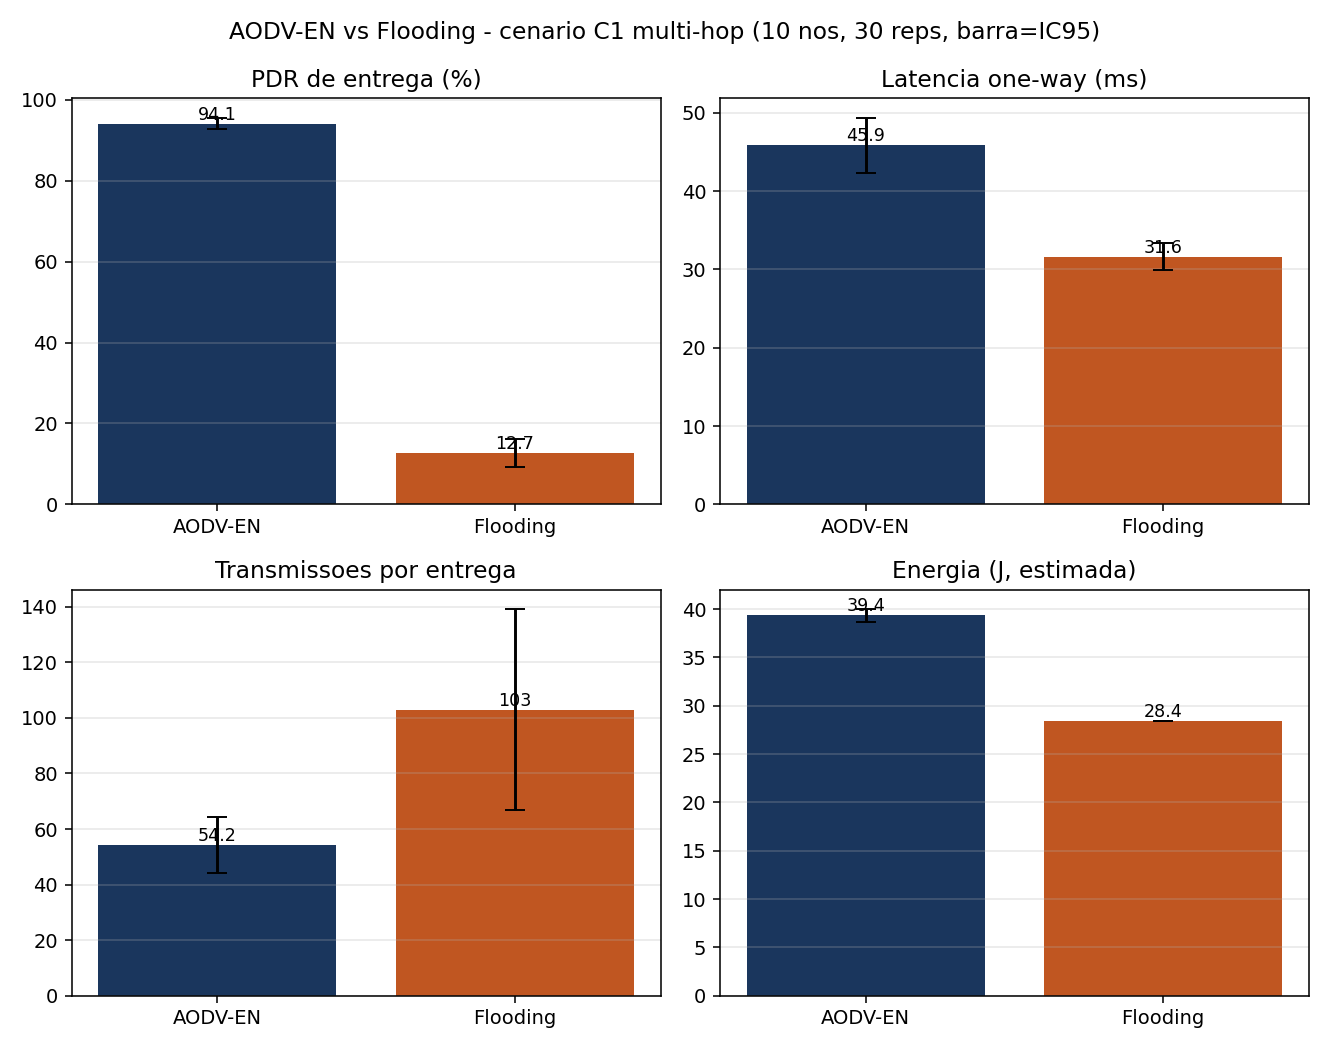
\includegraphics[keepaspectratio,alt={Métricas de hardware (PDR de entrega, latência, transmissões por entrega e energia): AODV-EN vs.~Flooding, média de 30 repetições com barra de IC95.}]{figuras/fig_hw_metrics.png}}
\caption{Métricas de hardware (PDR de entrega, latência, transmissões por
entrega e energia estimada): AODV-EN vs.~Flooding, cenário C1 multi-hop,
10 nós, média de 30 repetições com barra de IC95.}\label{fig:hw-metrics}
\end{figure}

\subsection{Significância estatística}\label{significuxe2ncia-estatuxedstica}

Para verificar se as diferenças observadas são estatisticamente
significativas, e não fruto da variabilidade amostral, aplicou-se a cada
métrica o teste $t$ de Welch (apropriado a variâncias desiguais) e, de
forma complementar, o teste não paramétrico de Mann--Whitney (que não
pressupõe normalidade), ambos bilaterais com nível de significância
$\alpha = 0{,}05$ e $n = 30$ repetições por algoritmo. A magnitude do
efeito foi quantificada pelo $d$ de Cohen. A Tabela~\ref{tab:stats}
resume os resultados.

\begin{table}[H]
\centering
\caption{Significância estatística das diferenças AODV-EN vs.~Flooding (cenário C1, $n=30$ por grupo)}\label{tab:stats}
\begin{tabular}{@{}lcccl@{}}
\toprule
Métrica & $t$ (Welch) & $p$ & $d$ de Cohen & Efeito \\
\midrule
PDR de entrega & 43,7 & $<0{,}001$ & 11,3 & altíssimo \\
Latência one-way & 7,2 & $<0{,}001$ & 1,85 & grande \\
NRL (controle/entregue) & 7,5 & $<0{,}001$ & 1,95 & grande \\
Transmissões por entrega & $-2{,}5$ & $0{,}011$ & $-0{,}71$ & médio \\
Energia (estimada) & 33,5 & $<0{,}001$ & 8,65 & altíssimo \\
\bottomrule
\end{tabular}

\vspace{2pt}
{\footnotesize Fonte: Elaborado pelos autores. Teste de Mann--Whitney concordante ($p<0{,}05$) em todas as métricas.}
\end{table}

Todas as diferenças são estatisticamente significativas ($p < 0{,}05$),
com os testes paramétrico e não paramétrico em concordância. Os tamanhos
de efeito da entrega ($d = 11{,}3$) e do consumo estimado ($d = 8{,}65$)
são muito superiores ao limiar convencional de efeito grande ($d > 0{,}8$),
indicando que a vantagem do AODV-EN na entrega multi-hop é estrutural, e
não marginal. A única diferença de efeito apenas médio é a de transmissões
por entrega ($d = -0{,}71$, $p = 0{,}011$), atenuada pela alta dispersão do
\emph{flooding} nessa métrica --- ainda assim significativa e desfavorável
ao \emph{flooding}.

\subsection{Distribuição entre repetições}\label{distribuiuxe7uxe3o-entre-repetiuxe7uxf5es}

A dispersão entre as repetições revela a \emph{estabilidade} de cada
algoritmo, informação que a média sozinha oculta. O AODV-EN entregou entre
85,2\% e 100\% dos pacotes (mediana 94,2\%; coeficiente de variação
$\mathrm{CV} = 4{,}2\%$), com apenas 4 das 30 repetições abaixo de 90\%. O
\emph{flooding}, em contraste, variou de 0\% a 36,2\% (mediana 10,7\%;
$\mathrm{CV} = 74{,}2\%$), com 20 das 30 repetições abaixo de 15\% e uma
repetição sem nenhuma entrega. A diferença de variabilidade --- CV de 4\%
contra 74\% --- mostra que o AODV-EN não apenas entrega mais, mas entrega de
forma previsível, ao passo que o \emph{flooding} colapsa de modo errático sob
as colisões da inundação a cada repetição.

\section{Discussão por Métrica}\label{discussuxe3o-por-muxe9trica}

\textbf{Confiabilidade (PDR).} No regime multi-hop (três a quatro
saltos), o AODV-EN entregou 94,1\% dos pacotes contra apenas 12,7\% do
\emph{flooding} --- diferença de grande magnitude e estatisticamente
inequívoca (intervalos de confiança disjuntos). O \emph{flooding} não
sobrevive ao multi-hop: sem rota nem retransmissão, cada pacote precisa
atravessar os saltos por difusão, e a probabilidade de sucesso decai
aproximadamente como o produto das probabilidades por enlace sob a
potência reduzida de 2~dBm. O descarte por TTL foi nulo, o que confirma
que a perda é de enlace --- colisões da tempestade de \emph{broadcast} e
ausência de confirmação --- e não de alcance fixo. O AODV-EN, ao
contrário, recupera perdas pela retransmissão fim-a-fim sobre a rota
estabelecida. A taxa de confirmação de ida e volta acentua o contraste
(91,7\% contra 3,7\%): além de entregar muito mais, o AODV-EN oferece
confirmação bidirecional confiável, propriedade ausente no
\emph{flooding}, cujo ACK também se difunde de volta e raramente completa
o trajeto de retorno. A Figura~\ref{fig:pdr-rep} evidencia, repetição a
repetição, a entrega alta e estável do AODV-EN frente à entrega baixa e
dispersa do \emph{flooding}.

\begin{figure}
\centering
\pandocbounded{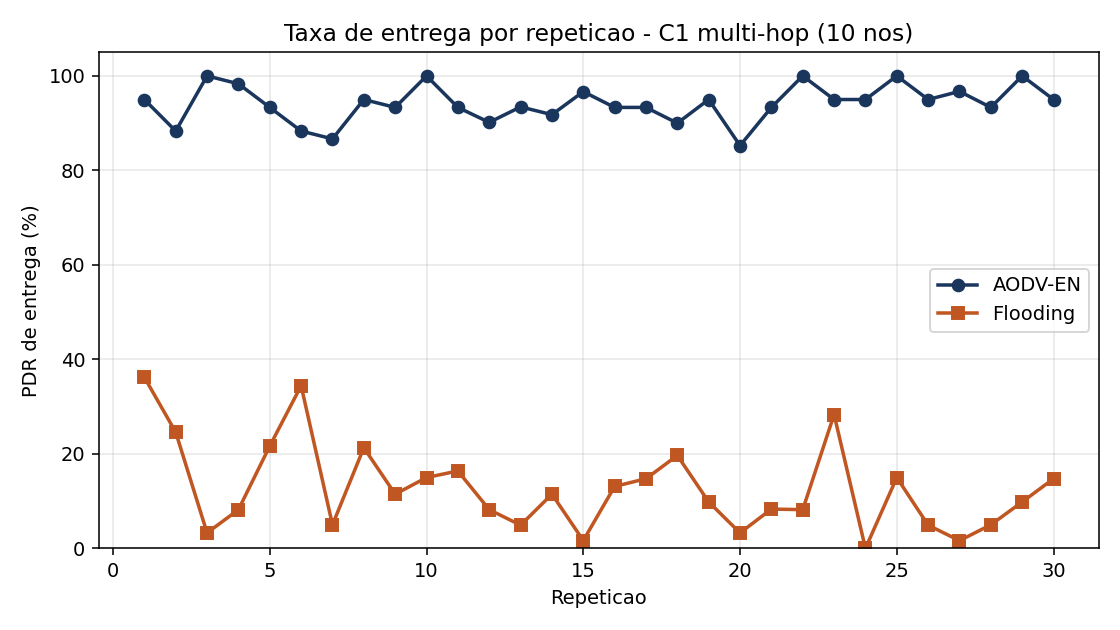
\includegraphics[keepaspectratio,alt={Taxa de entrega (PDR) por repetição: AODV-EN alto e estável (~94\%) frente ao flooding baixo e disperso (~13\%).}]{figuras/fig_pdr_rep.png}}
\caption{Taxa de entrega por repetição (AODV-EN vs.~Flooding), cenário C1
multi-hop, 10 nós.}\label{fig:pdr-rep}
\end{figure}

\textbf{Latência fim-a-fim.} A latência one-way do \emph{flooding}
(31,6 ms) foi menor que a do AODV-EN (45,9 ms), mas o número não
representa vantagem: trata-se de viés de sobrevivência. No \emph{flooding}
apenas a pequena fração de pacotes que percorre caminhos curtos e pouco
congestionados sobrevive, e são justamente esses os que entram na média;
o AODV-EN entrega também os pacotes de caminho mais longo, que elevam a
média. Medida na própria origem por RTT no relógio de microssegundos
(\emph{esp\_timer}), a latência não sofre a quantização por laço de
aplicação presente em versões anteriores do protótipo.

\textbf{Carga de roteamento e custo de canal.} A NRL clássica (mensagens
de controle de rota por dado entregue) foi 18,0 para o AODV-EN e nula
para o \emph{flooding}, que não possui plano de roteamento. Esse contraste,
isoladamente, não deve ser interpretado como ausência de custo: o
\emph{flooding} não paga \emph{overhead} de controle de rota, mas seu custo
desloca-se para as retransmissões por inundação, que a NRL não contabiliza. A métrica justa é o total de transmissões por pacote
entregue: 54,2 para o AODV-EN contra 102,9 para o \emph{flooding} ---
isto é, mesmo somando todo o controle de rota, o AODV-EN custa cerca de
metade das transmissões por pacote efetivamente entregue. Esse valor do
\emph{flooding} é, ainda, subestimado: apenas sete dos dez nós
conseguiram reportar telemetria de volta ao coletor (a própria difusão de
relatórios é perdida), de modo que parte das retransmissões não foi
contabilizada.

\textbf{Consumo energético.} O consumo agregado estimado da rede foi
maior no AODV-EN (39,4 J) que no \emph{flooding} (28,4 J) na janela --- mas
esse número \emph{bruto} pode induzir a uma conclusão equivocada, por duas razões: a comparação não está
em pé de igualdade (o AODV-EN manteve nove nós ativos com HELLO periódico e
encaminhamento, enquanto o \emph{flooding} teve apenas sete nós
contabilizados e não emite HELLO) e, sobretudo, ele ignora que o AODV-EN
entrega muito mais. A métrica justa é a \emph{energia por pacote efetivamente
entregue}: 0,69~J/pacote para o AODV-EN contra 5,66~J/pacote para o
\emph{flooding} --- ou seja, o AODV-EN é cerca de \textbf{8 vezes mais
eficiente em energia por entrega útil}. O \emph{flooding} gasta energia
disseminando pacotes que, em sua maioria, não sobrevivem ao multi-hop. Cabe
ressalvar que todos os valores de energia são \emph{estimados} a partir do
perfil de \emph{datasheet} do ESP32, não medidos com instrumentação física;
ainda assim, como a estimativa usa os mesmos coeficientes para os dois
algoritmos, a razão entre eles é robusta à incerteza absoluta do modelo.

\section{Cenário de Malha Densa (C3)}\label{cenario-de-malha-densa-c3}

O cenário C1 avaliou uma topologia em cadeia (caminho essencialmente
único). Para verificar se as conclusões se sustentam em uma topologia
\emph{não linear}, com caminhos redundantes, conduziu-se o cenário C3: dez
módulos ESP32 espalhados ao máximo em um apartamento, formando uma malha de
maior profundidade (cinco saltos). De forma deliberada, manteve-se o mesmo
\emph{firmware} e a mesma potência de transmissão do C1 (2~dBm), de modo que
a comparação isola o efeito da \emph{topologia}: cadeia (C1) contra malha
(C3), nas mesmas demais condições. A Tabela~\ref{tab:c3} consolida os
resultados de 30 repetições por algoritmo.

\begin{table}[H]
\centering
\caption{Comparação AODV-EN vs.~Flooding no cenário C3 (malha densa, 10 nós, 5 saltos, 30 repetições; média $\pm$ IC95)}\label{tab:c3}
\begin{tabular}{@{}lcc@{}}
\toprule
Métrica & AODV-EN & Flooding \\
\midrule
PDR de entrega (\%) & 91,4 $\pm$ 2,2 & 77,8 $\pm$ 3,7 \\
Latência one-way (ms) & 34,9 $\pm$ 2,7 & 20,5 $\pm$ 0,6 \\
Transmissões por entrega & 42,6 $\pm$ 2,7 & 33,3 $\pm$ 1,7 \\
Recepções por entrega (canal) & 55,7 $\pm$ 2,5 & 86,4 $\pm$ 5,4 \\
Energia por pacote entregue (J) & 0,70 $\pm$ 0,02 & 0,83 $\pm$ 0,05 \\
\bottomrule
\end{tabular}

\vspace{2pt}
{\footnotesize Fonte: Elaborado pelos autores. Todas as diferenças são significativas (teste $t$ de Welch, $p<0{,}001$).}
\end{table}

O resultado mais relevante é o contraste com o C1. Na malha densa, o
\emph{flooding} \emph{não colapsa} como na cadeia fina: a redundância de
caminhos eleva sua entrega a 77,8\%, contra apenas 12,7\% no C1. O AODV-EN
ainda entrega significativamente mais (91,4\% contra 77,8\%; $t = 6{,}19$,
$p < 0{,}001$, $d = 1{,}6$), mas a sua vantagem de confiabilidade
\emph{encolhe} --- de cerca de 81 pontos percentuais no C1 para 13 pontos no
C3. A Figura~\ref{fig:topology-dependence} sintetiza esse achado central: a
vantagem do roteamento sobre a inundação é \emph{dependente da topologia},
máxima em redes esparsas ou em cadeia e modesta em malhas densas, nas quais a
própria redundância do \emph{flooding} o torna competitivo em entrega.

\begin{figure}
\centering
\pandocbounded{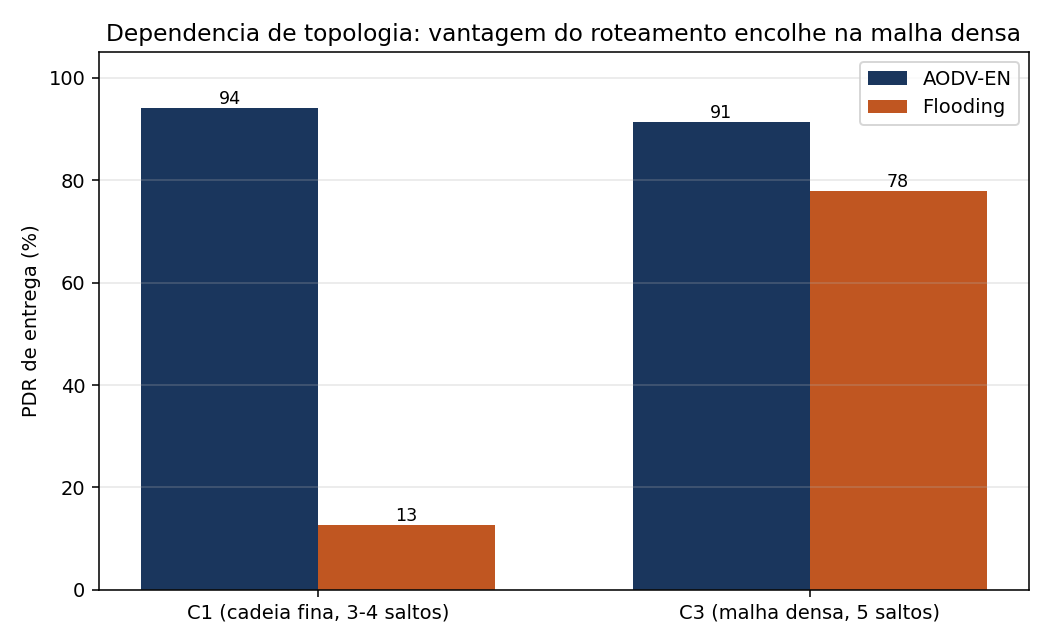
\includegraphics[keepaspectratio,alt={PDR do AODV-EN e do flooding nos cenarios C1 (cadeia) e C3 (malha): na malha o flooding recupera e o gap encolhe.}]{figuras/fig_topology_dependence.png}}
\caption{Dependência de topologia: o \emph{flooding} colapsa na cadeia fina
(C1) mas recupera na malha densa (C3) graças à redundância de caminhos,
estreitando a vantagem de entrega do AODV-EN.}\label{fig:topology-dependence}
\end{figure}

A vantagem do AODV-EN, contudo, persiste em duas dimensões que a entrega
isolada não revela (Figura~\ref{fig:c3-compare}). Primeiro, a \emph{ocupação
de canal}: cada pacote entregue pelo \emph{flooding} custa 86,4 recepções
agregadas na rede, contra 55,7 do AODV-EN --- consequência da tempestade de
\emph{broadcast}, em que cada disseminação é ouvida por todos os vizinhos.
Segundo, a \emph{energia por pacote entregue}, menor no AODV-EN (0,70 contra
0,83~J). A menor latência do \emph{flooding} (20,5 contra 34,9~ms) reflete,
novamente, viés de sobrevivência e o uso do caminho de difusão mais curto.
Em síntese, mesmo onde o \emph{flooding} entrega bem, o AODV-EN o supera em
entrega e em custo de canal por pacote útil.

\begin{figure}
\centering
\pandocbounded{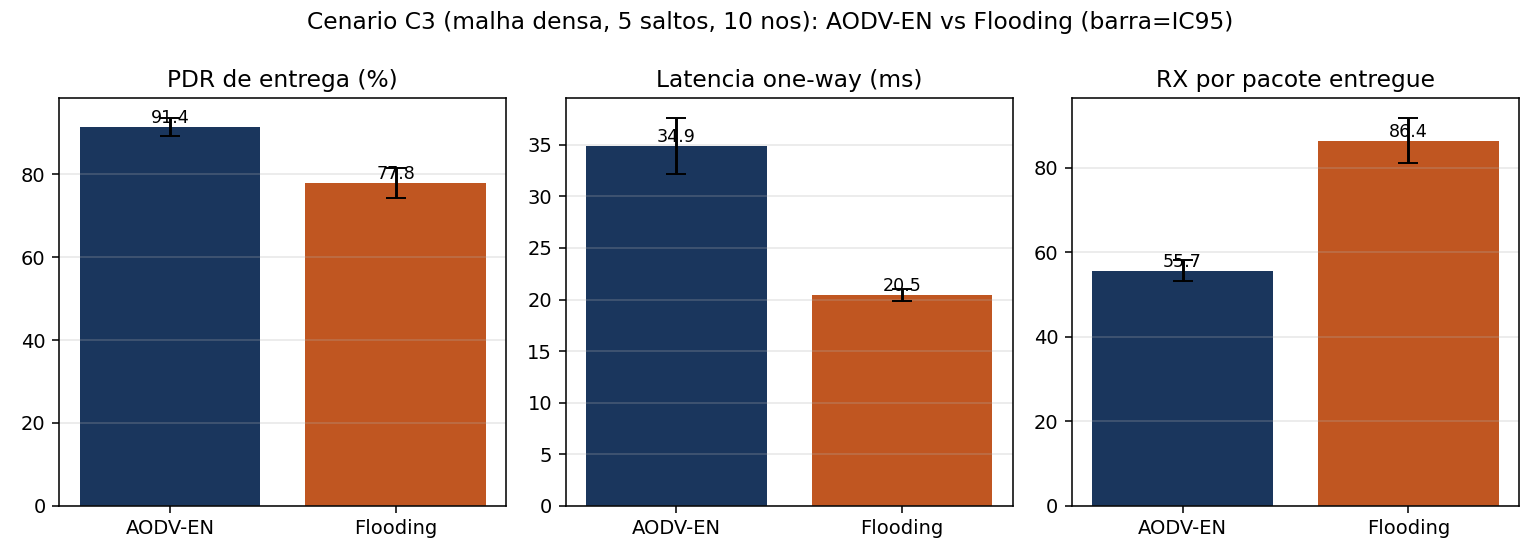
\includegraphics[keepaspectratio,alt={AODV-EN vs flooding no cenario C3: PDR, latencia e recepcoes por entrega.}]{figuras/fig_c3_compare.png}}
\caption{Cenário C3 (malha densa): AODV-EN vs.~Flooding em entrega, latência e
recepções por pacote entregue (ocupação de canal), com barra de IC95.}\label{fig:c3-compare}
\end{figure}

\section{Cenário de Falha e Auto-recuperação (C4)}\label{cenario-de-falha-c4}

Para avaliar especificamente a capacidade de recuperação do protocolo diante
da perda de um nó, conduziu-se o cenário C4 em hardware, em uma topologia
distinta da do cenário C1. Foram empregados seis módulos ESP32 distribuídos
em um apartamento, com potência de transmissão de 4~dBm --- maior que a do C1
(2~dBm) em razão do espaço menor e da maior densidade de paredes, mantida a
verificação por RSSI. A origem (também coletor) transmite ao destino por meio
de um relé \emph{on-path}, que dispõe de um relé alternativo. A falha é
induzida por \emph{firmware}: o relé do caminho principal silencia o rádio
por 15~s a cada 45~s (33\% de indisponibilidade), simulando a queda e o
retorno cíclicos do nó; os vizinhos detectam a quebra pelas mensagens HELLO,
emitem RERR e o AODV-EN re-descobre a rota pelo relé alternativo.

A Tabela~\ref{tab:c4} consolida as métricas do cenário C4 ao longo de 30
repetições (média $\pm$ IC95).

\begin{table}[H]
\centering
\caption{Métricas do AODV-EN no cenário C4 (falha induzida, 6 nós, 30 repetições; média $\pm$ IC95)}\label{tab:c4}
\begin{tabular}{@{}lc@{}}
\toprule
Métrica & AODV-EN sob falha \\
\midrule
PDR de entrega (\%) & 62,8 $\pm$ 11,5 \\
PDR confirmação ida-volta (\%) & 47,6 $\pm$ 11,5 \\
Latência one-way (ms) & 60,7 $\pm$ 14,6 \\
NRL (controle de rota/entregue) & 5,2 $\pm$ 1,7 \\
Energia (J, estimada) & 9,2 $\pm$ 1,7 \\
\bottomrule
\end{tabular}

\vspace{2pt}
{\footnotesize Fonte: Elaborado pelos autores. NRL e energia não são diretamente comparáveis às do C1 por diferirem o número de nós (6 vs.~10) e a topologia.}
\end{table}

\textbf{Impacto da falha.} Em relação ao mesmo protocolo \emph{sem} falha
(cenário C1, 94,1\%), a taxa de entrega caiu para 62,8\% --- uma redução de
cerca de 31 pontos percentuais, estatisticamente significativa (teste $t$ de
Welch: $t = 5{,}3$, $p < 0{,}001$; $d$ de Cohen $= 1{,}37$, efeito grande). A
latência subiu de 45,9~ms para 60,7~ms ($t = -1{,}94$, $p = 0{,}05$),
refletindo o tempo de detecção da quebra (\emph{timeout} de HELLO) somado à
re-descoberta de rota. A Figura~\ref{fig:c4-metrics} contrasta as duas
condições.

\begin{figure}
\centering
\pandocbounded{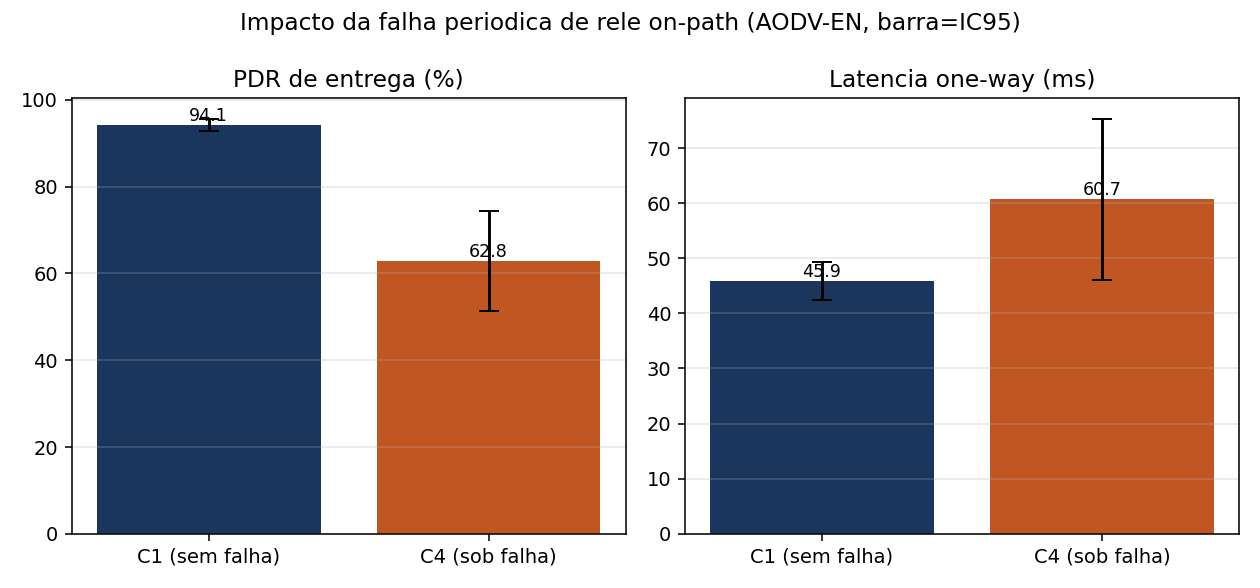
\includegraphics[keepaspectratio,alt={Comparacao do PDR e da latencia do AODV-EN entre o cenario C1 (sem falha) e o C4 (sob falha), com barras de IC95.}]{figuras/fig_c4_metrics.png}}
\caption{Impacto da falha periódica de um relé \emph{on-path}: PDR de entrega
e latência do AODV-EN no cenário C1 (sem falha) contra o C4 (sob falha), com
barra de IC95.}\label{fig:c4-metrics}
\end{figure}

\textbf{Distribuição e variabilidade.} A entrega no C4 variou de 0\% a 100\%
entre as repetições (mediana 73,3\%; coeficiente de variação de 51\%): 12 das
30 repetições preservaram entrega $\geq 80\%$, enquanto 8 ficaram abaixo de
40\%. Essa dispersão (Figura~\ref{fig:c4-pdr-rep}) decorre da natureza
estocástica do instante da falha em relação ao tráfego --- repetições em que a
janela de queda coincide com poucos envios preservam entrega alta, enquanto
outras concentram as perdas no intervalo de recuperação.

\begin{figure}
\centering
\pandocbounded{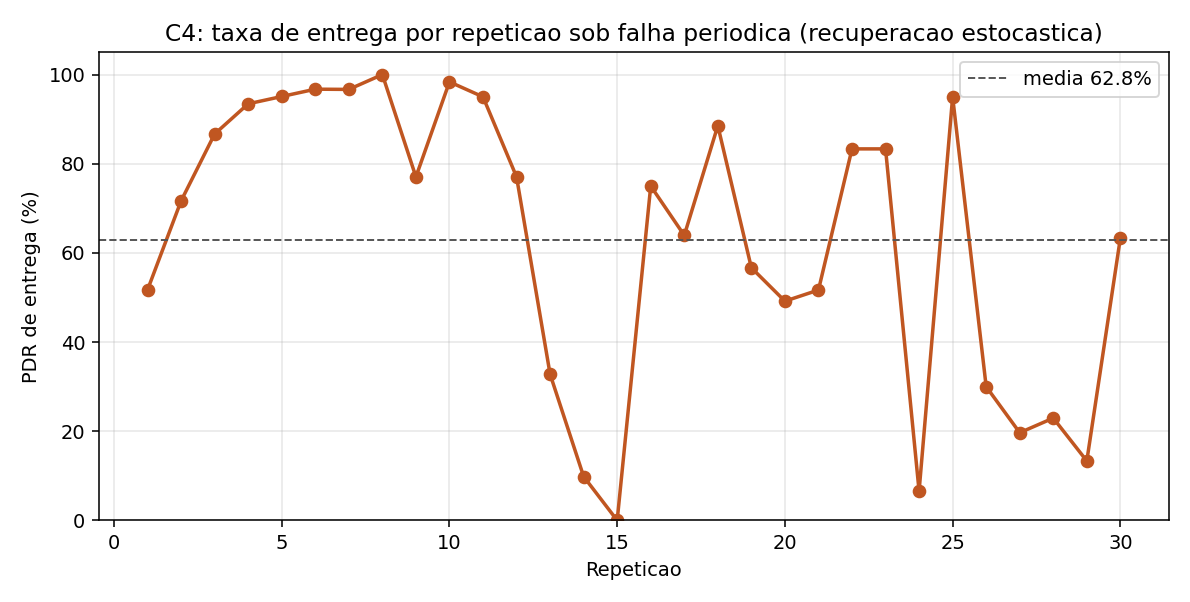
\includegraphics[keepaspectratio,alt={Taxa de entrega por repeticao no cenario C4, evidenciando a variabilidade da recuperacao sob falha.}]{figuras/fig_c4_pdr_rep.png}}
\caption{Taxa de entrega por repetição no cenário C4: a alta variabilidade
reflete a recuperação estocástica diante da falha periódica do relé.}\label{fig:c4-pdr-rep}
\end{figure}

\textbf{Dinâmica da recuperação.} A Figura~\ref{fig:c4-selfheal} ilustra o
mecanismo em uma repetição: a curva de pacotes entregues acumulados exibe
\emph{patamares} --- intervalos sem entrega que coincidem com a
indisponibilidade do relé --- seguidos de \emph{retomada}, evidência direta da
auto-recuperação (\emph{self-healing}) pela rota alternativa.

\begin{figure}
\centering
\pandocbounded{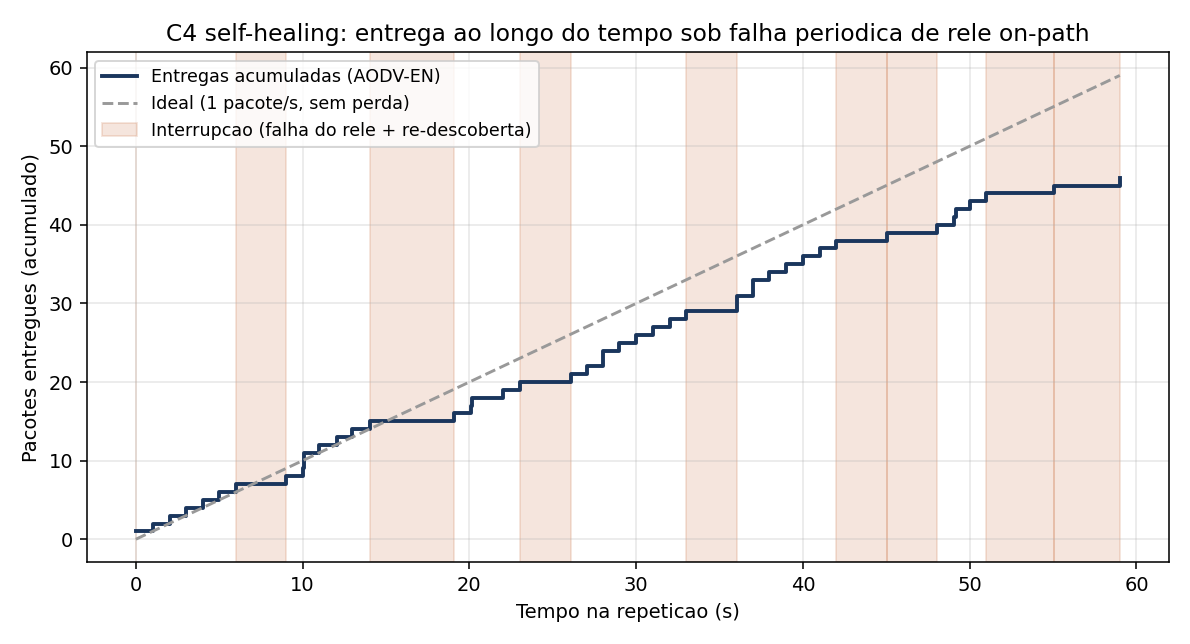
\includegraphics[keepaspectratio,alt={Entregas acumuladas ao longo do tempo em uma repeticao do cenario C4: patamares coincidem com a falha do rele e a retomada evidencia a recuperacao.}]{figuras/fig_c4_selfheal.png}}
\caption{Auto-recuperação no cenário C4: pacotes entregues acumulados ao longo
de uma repetição. Os patamares (faixas destacadas) coincidem com a queda do
relé \emph{on-path}; a retomada da entrega evidencia a re-descoberta de rota
pelo relé alternativo.}\label{fig:c4-selfheal}
\end{figure}

Esse resultado expõe, de forma honesta, o \emph{trade-off} entre eficiência e
resiliência. O roteamento reativo do AODV-EN é eficiente em condições
estáveis (Seção~\ref{resultados-de-hardware}), mas paga um custo de detecção e
re-descoberta quando um nó do caminho falha. A inundação, por não manter
rotas, é estruturalmente tolerante à queda de um nó isolado --- a difusão
simplesmente contorna o nó ausente ---, porém ao preço da ocupação de canal
já discutida e da baixa entrega em múltiplos saltos. Assim, a escolha entre as
abordagens depende do regime de operação: redes estáveis e maiores favorecem o
roteamento; cenários de altíssima volatilidade de nós, sem exigência de
eficiência de banda, podem tolerar a inundação. A avaliação quantitativa do
\emph{flooding} sob o mesmo padrão de falha, sobre a infraestrutura já
preparada, constitui extensão direta deste trabalho.

\section{Análise de Escalabilidade por
Simulação}\label{anuxe1lise-de-escalabilidade-por-simulauxe7uxe3o}

Para estender a avaliação a topologias além da cadeia de dez nós
medida em hardware, conduziu-se uma varredura por simulação em grades de
4 a 25 nós, medindo o número de transmissões por pacote entregue. A
Figura~\ref{fig:sim-crossover} apresenta o resultado: ambos os algoritmos
entregam a totalidade dos pacotes dentro do alcance do TTL, mas a razão
transmissões-por-entrega cruza-se em torno de 9 a 11 nós, acima do qual o
roteamento do AODV-EN passa a custar menos transmissões por entrega que o
\emph{flooding}. Além disso, com o TTL limitado a cinco saltos, o
\emph{flooding} deixa de alcançar destinos em grades de diâmetro superior
a cinco --- limitação estrutural do alcance fixo ---, enquanto o AODV-EN,
por manter rotas, continua entregando. A simulação assume enlaces ideais
dentro do alcance; o experimento em hardware (Seção~\ref{resultados-de-hardware}),
sob enlaces reais a 2~dBm e perda por colisão, mostra que a vantagem do
roteamento se manifesta ainda mais cedo, já na cadeia de dez nós.

\begin{figure}
\centering
\pandocbounded{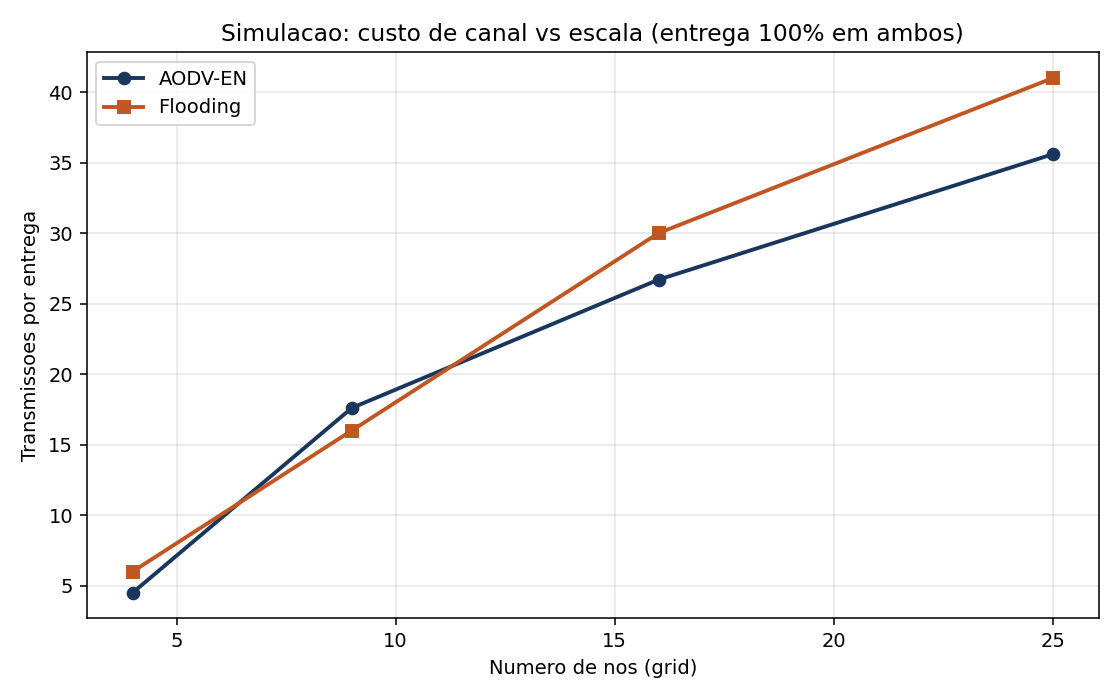
\includegraphics[keepaspectratio,alt={Transmissões por pacote entregue em função do número de nós (simulação).}]{figuras/fig_sim_crossover.png}}
\caption{Transmissões por pacote entregue em função do
número de nós (simulação).}
\label{fig:sim-crossover}
\end{figure}

Esse resultado confirma a hipótese central do trabalho: o roteamento
reativo paga um \emph{overhead} de controle aproximadamente constante
para evitar o custo de disseminação que cresce com a rede. Já na cadeia
multi-hop de dez nós em hardware, o AODV-EN entrega 7,4 vezes mais
pacotes com cerca de metade das transmissões por entrega; a sua vantagem
estrutural amplia-se à medida que a rede cresce em tamanho e diâmetro.

\section{Comparação com Trabalhos Correlatos}\label{comparacao-literatura}

A Tabela~\ref{tab:literatura} posiciona o AODV-EN frente a soluções
representativas da literatura para comunicação sobre ESP-NOW. A comparação deve
ser interpretada com cautela, pois as condições experimentais --- topologia,
ambiente, distância e número de nós --- diferem entre os trabalhos; ainda assim,
situa o desempenho do AODV-EN em ordem de grandeza compatível e evidencia seu
diferencial de ser a única abordagem fundamentada em um protocolo de roteamento
padronizado (AODV, RFC 3561).

{\def\LTcaptype{table}
\begin{longtable}[]{@{}
  >{\raggedright\arraybackslash}p{(\linewidth - 6\tabcolsep) * \real{0.2600}}
  >{\raggedright\arraybackslash}p{(\linewidth - 6\tabcolsep) * \real{0.3200}}
  >{\centering\arraybackslash}p{(\linewidth - 6\tabcolsep) * \real{0.1200}}
  >{\raggedright\arraybackslash}p{(\linewidth - 6\tabcolsep) * \real{0.3000}}@{}}
\caption{Comparação do AODV-EN com trabalhos correlatos sobre ESP-NOW}\label{tab:literatura}\\
\toprule\noalign{}
Trabalho & Base de roteamento & PDR & Latência / condição \\
\midrule\noalign{}
\endfirsthead
\toprule\noalign{}
Trabalho & Base de roteamento & PDR & Latência / condição \\
\midrule\noalign{}
\endhead
\bottomrule\noalign{}
\endlastfoot
AODV-EN (este trabalho) & AODV reativo padronizado (RFC 3561), multi-hop & 94,1\% & $\approx$46~ms; 10 nós, multi-hop real em hardware (3--4 saltos) \\
BRAM-NOW \cite{cujilema2023} & Mesh \emph{ad-hoc} não padronizado & $\approx$90,8\%\textsuperscript{b} & 75~ms; residencial, multi-hop \\
ESP-NOW base \cite{becker2025} & Ponto-a-ponto (sem roteamento) & $>$99\% & 2,8~ms/salto; campo aberto, linha de visada \\
\end{longtable}
}

Fonte: Elaborado pelos autores.

\noindent\footnotesize\textsuperscript{b}Complemento da taxa de perda de 9,25\% reportada pelos autores.
\normalsize

No regime avaliado, o AODV-EN apresentou confiabilidade superior à do BRAM-NOW
(94,1\% contra $\approx$90,8\%) sob topologia multi-hop real de três a quatro
saltos, mantendo latência da mesma ordem de grandeza; a avaliação em escalas
ainda maiores foi complementada por simulação
(Seção~\ref{anuxe1lise-de-escalabilidade-por-simulauxe7uxe3o}). Frente ao ESP-NOW
puro \cite{becker2025}, o custo adicional de latência decorre do plano de
roteamento e do multi-hop, e não do meio físico. O principal
diferencial do AODV-EN é apoiar-se em um protocolo padronizado e amplamente
documentado, propriedade ausente nas soluções \emph{ad-hoc} correlatas, o que
favorece reprodutibilidade, comparabilidade e extensões futuras.

\section{Conformidade com a RFC 3561}\label{conformidade-com-a-rfc-3561}

Ao longo do desenvolvimento, o núcleo do protocolo foi submetido a uma
auditoria de conformidade com a RFC 3561, da qual resultaram ajustes
pontuais. Destacam-se: (i) a deduplicação de mensagens DATA no destino,
por par (originador, número de sequência), evitando entregas repetidas
em caso de retransmissão por expiração de ACK, com reconfirmação
idempotente; (ii) a contabilização de confirmações apenas quando
associadas a um envio pendente vivo, eliminando dupla contagem; (iii) o
processamento de mensagens RERR condicionado a que o próximo salto da
rota corresponda ao vizinho que emitiu o erro, conforme a Seção 6.11 da
RFC 3561 \cite{perkins2003}, com adoção do número de sequência informado; (iv) a manutenção de
rotas invalidadas por um período de exclusão (\emph{delete period})
antes de sua remoção, preservando o último número de sequência
conhecido; e (v) a proteção contra o rebaixamento de uma rota confirmada
por uma entrada reversa não confirmada. Tais ajustes aproximam a
implementação do comportamento especificado e aumentam a robustez do
protocolo em cenários com perda de enlace.

\section{Escopo Implementado e
Limitações}\label{escopo-implementado-e-limitauxe7uxf5es}

A avaliação reportada refere-se ao núcleo reativo do AODV-EN ---
descoberta de rotas sob demanda, tabelas de rota com números de
sequência, precursores, fila de dados pendentes, confirmação fim-a-fim e
invalidação por falha de enlace --- utilizando disseminação de RREQ por
\emph{broadcast} e métrica de contagem de saltos. As adaptações de
gerenciamento de \emph{peers} por política LRU e de métrica híbrida
(saltos + RSSI), embora projetadas e implementadas no \emph{firmware}
(Capítulo~\ref{cap:implementacao}), não foram objeto de um experimento
dedicado de isolamento: o cenário C1 multi-hop já aproxima o coletor do
limite do \emph{cache} de \emph{peers} e exercita a seleção de rota sobre
múltiplos saltos, mas a aferição específica do efeito da substituição por
LRU e do ganho da métrica híbrida sobre a contagem de saltos pura permanece
como objeto de trabalhos futuros, em topologias mais densas e com variação
deliberada de RSSI por enlace.

As principais limitações do estudo são: (i) a cobertura de cenários ---
a campanha em hardware cobre os cenários C1 (cadeia de dez nós), C3 (malha
densa de dez nós, cinco saltos) e C4 (falha induzida, seis nós), todos com
trinta repetições por algoritmo, e a avaliação quantitativa do \emph{flooding}
sob falha (C4) e o cenário C2 (árvore hierárquica), embora viabilizados pela
mesma infraestrutura de coleta, ficam como trabalho
futuro; (ii) o caráter estimado do
consumo energético, calculado a partir do perfil de \emph{datasheet} do
ESP32 e não medido com instrumentação física --- a medição direta de
corrente (por exemplo, com um sensor INA219 em série com a alimentação) é
registrada como trabalho futuro; e (iii) o fato de as campanhas do
AODV-EN e do \emph{flooding} terem sido coletadas em sequência, com
reprogramação e nova distribuição física dos nós entre elas, o que
introduz pequena variação de topologia e de condições de canal; soma-se a
isso que, na campanha de \emph{flooding}, parte da telemetria de rede não
retornou ao coletor (sete dos dez nós), subestimando as métricas de custo
agregado desse algoritmo. A medição física de energia, a execução do
cenário C2 (árvore) e a avaliação do \emph{flooding} sob falha constituem
desdobramentos diretos para trabalhos futuros.
